\subsection{Solenoid}
\label{sec:solenoid}

As its name suggests, a central feature of the CMS 
detector is a large, superconducting solenoid.  
Large bending power (i.e. a large magnetic field) 
is necessary in order to unambiguously determine the sign of the electric charge 
of muons with momentum greater than 1 TeV.  This requirement forced the choice
of a superconducting technology for the solenoid.
In addition, the solenoid was designed to contain both the inner tracking 
and calorimetry detector subsystems, while maintaining a favorable 
length-to-diameter ratio in order to ensure good track momentum resolution
in the forward region.
The nominal specifications are for a 4 T field
with 2.6 GJ of stored energy at full current in
a free bore of 6 m diameter and a length of 12.5 m.
In practice, the solenoid produces a magnetic field of 3.8 T with 
2.35 GJ of stored energy.
The flux is returned via a 10,000 ton iron return yoke made up
of 5 wheels and two endcaps.  Each endcap is composed of three disks.
The solenoid is made up of five separate sections and placed within a cryostat,
as shown in Figure \ref{fig:solenoid}.
The cryostat is cooled to 4.5 K in order to maintain superconductivity.
Other design parameters for the solenoid are given in Table
\ref{tab:solenoid}.  

\begin{figure}
  \centering
  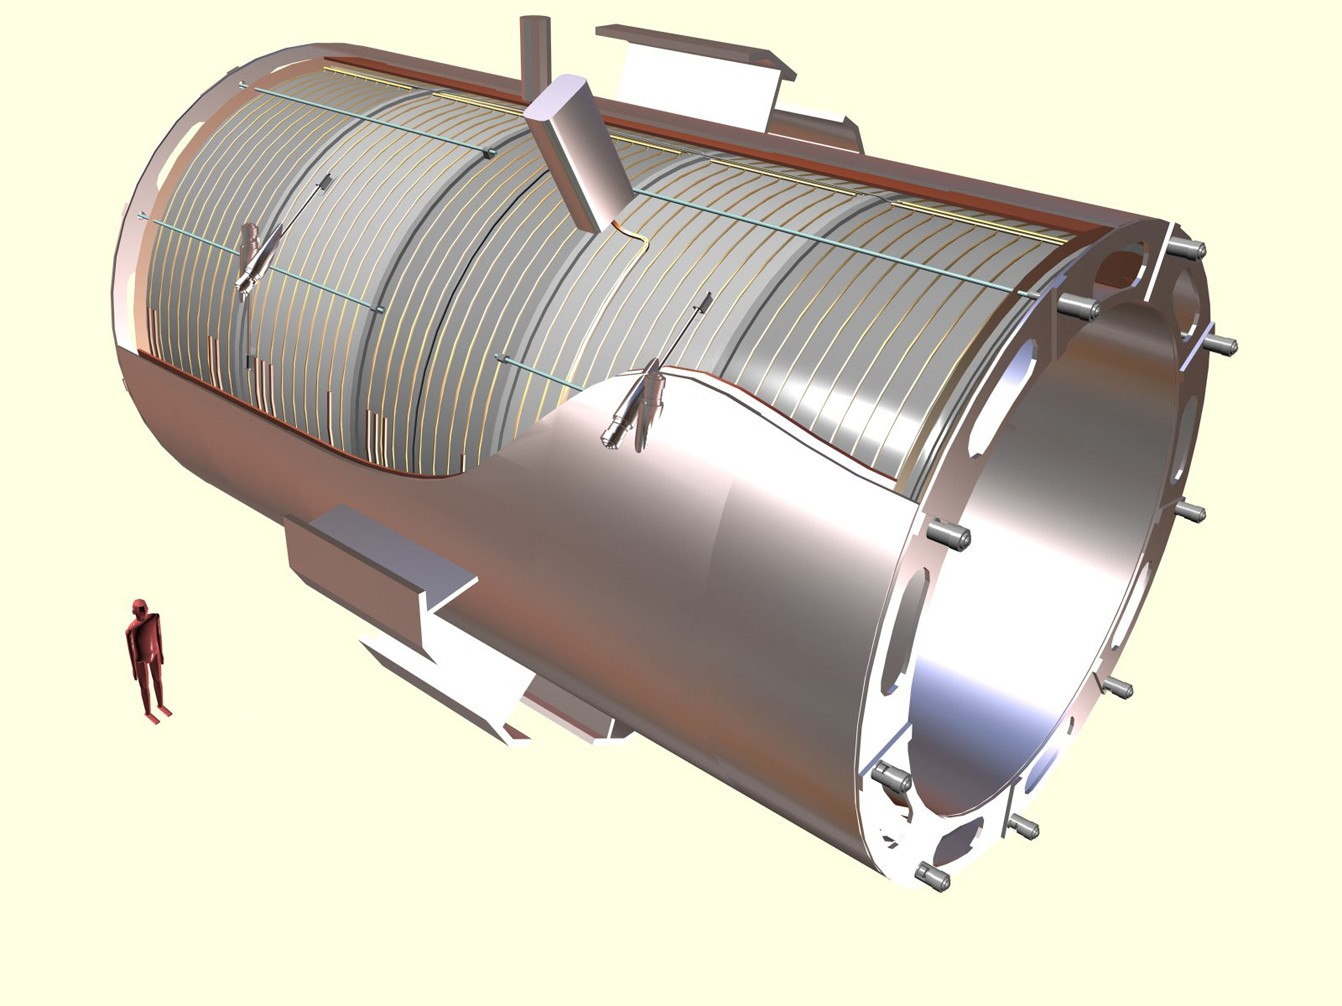
\includegraphics[width=0.6\textwidth]{tex/cms/fig/magnet-schematic.jpg}
  \caption{Artistic representation of the CMS solenoid.  The outer layer (cryostat)
    has been cut away to show the solenoid's five individual sections. \cite{cms-jinst}.}
  \label{fig:solenoid}
\end{figure}

\begin{table}
  \begin{tabular}{c|c}
    \multicolumn{2}{c}{General parameters} \\
    \hline\hline
    Magnetic length & 12.5 m \\
    Cold bore diameter & 6.3 m \\
    Central magnetic induction & 4 T \\
    Total Ampere-turns & 41.7 MA-turns \\ 
    Nominal current Z & 19.14 kA \\
    Inductance & 14.2 H \\
    Stored energy & 2.6 GJ \\
    \hline\hline
    \multicolumn{2}{c}{Cold mass} \\
    \hline\hline
    \multirow{2}{*}{Layout} & Five modules mechanically and \\ 
    & electrically coupled \\ 
    Radial thickness of cold mass & 312 mm \\
    Radiation thickness of cold mass & 3.9 $X_0$ \\ 
    Weight of cold mass & 220 t \\
    Maximum induction on conductor & 4.6 T \\ 
    Temperature margin wrt operating temperature & 1.8 K \\
    Stored energy/unit cold mass & 11.6 kJ/kg \\
    \hline\hline
    \multicolumn{2}{c}{Iron yoke} \\
    \hline\hline
    Outer diameter of the iron flats & 14 m \\ 
    Length of barrel & 13 m \\
    Thickness of the iron layers in barrel & 300, 630 and 630 mm \\
    Mass of iron in barrel & 6000 t \\
    Thickness of iron disks in endcaps & 250, 600, and 600 mm \\ 
    Mass of iron in each endcap & 2000 t \\ 
    Total mass of iron in return yoke & 10000 t \\
  \end{tabular}
  \caption{Design parameters of the CMS solenoid \cite{cms-jinst}}
  \label{tab:solenoid} 
\end{table}

The CMS solenoid has several features that are distinctive relative to the
solenoids used in previous particle detectors.  First,
due to the large number of ampere turns needed to generate a 4 T field 
(41.7 MA-turn), the CMS solenoid winding has four layers instead of the usual single layer.
Second, the conductor is made from a Rutherford-type cable of NbTi co-extruded
with pure aluminum and mechanically reinforced with an aluminum alloy.
Finally, the ratio between the nominal stored energy (2.6 GJ) and the nominal 
effective cold coil mass (220 t) is significantly higher for the CMS solenoid
than for solenoids of previous detectors, as shown in Figure \ref{fig:solenoid-comparison}.
This leads to a 0.15\% mechanical deformation during energizing \cite{cms-jinst,cms-tdr}.

\begin{figure}
  \centering
  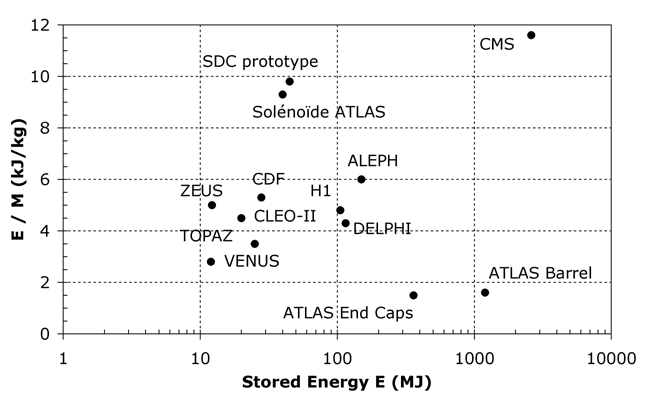
\includegraphics[width=0.8\textwidth]{tex/cms/fig/magnet-comparison.png}
  \caption{
    Comparison between the CMS solenoid and various other detector magnets.
    The x-axis (log scale) corresponds to the stored energy, $E$, of the magnet in units of MJ.
    The y-axis corresponds to the ratio between nominal stored energy and nominal effective cold coil mass of the magnet, $E/M$
    in units of $\text{kJ}/\text{kg}$.
    The CMS solenoid surpasses all of the other magnets displayed here 
    with respect to both variables \cite{cms-jinst}.
  }
  \label{fig:solenoid-comparison}
\end{figure}

